\subsubsection{Experiments}
\label{sec:view_experiment}

\paragraph{}
Before a user can do anything in ROME, they need to create an experiment. The main page for managing experiments is linked under the Session tab of the menu and provides the user with an interface to create new experiments and manage existing ones. The basis structure of the page is illustrated in figure \ref{fig:experiment_page_structure}


\begin{figure}[h]
\centering
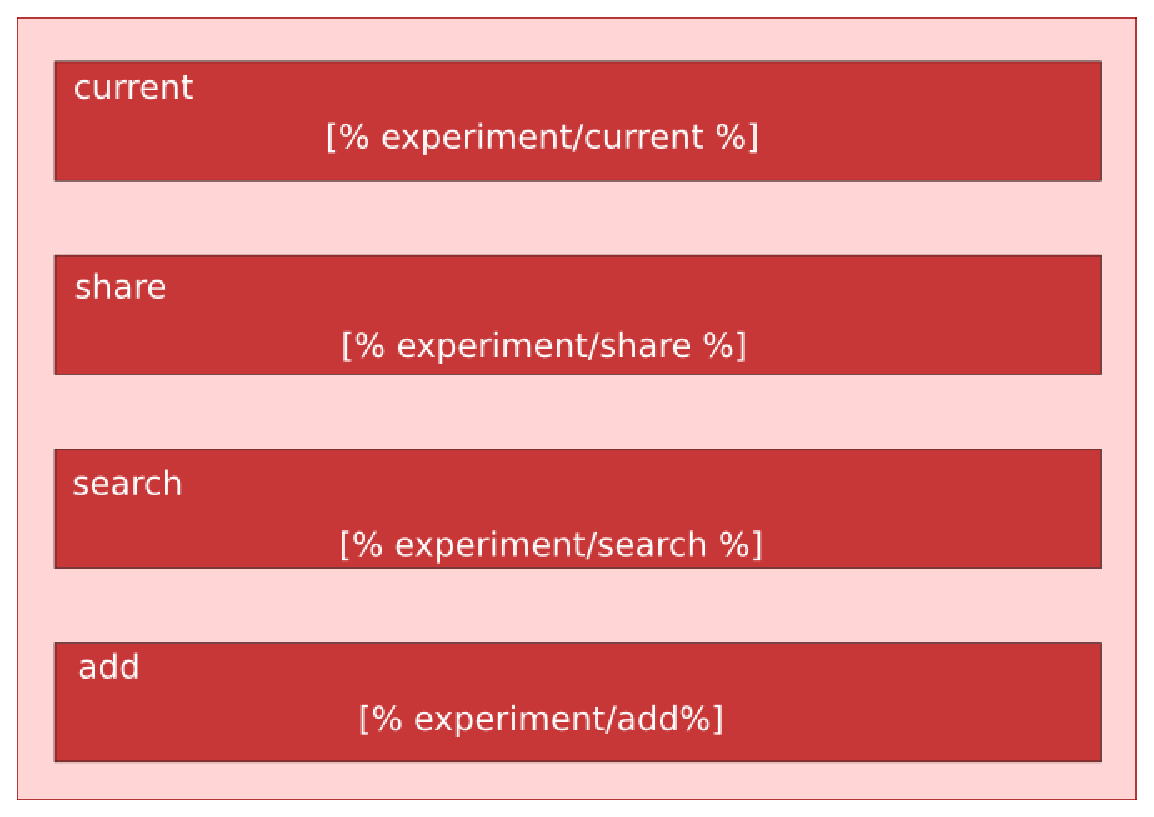
\includegraphics[scale=0.6]{../rome/docs/images/experiment_page_structure}
\caption{Structure of the Expeirment Page}\label{fig:experiment_page_structure}
\end{figure}

\paragraph{}
The current experiment section provides basic details about the experiment the user currently has selected. The controller provides an AJAX action to update this section if the selected experiment changes without a page reload. The share experiment form allows the user to select from their existing experiments (the experiment field is an AJAX autocompleter and will return a list of suggestions as the user types) and share them with everyone or with selected workgroups. The experiment search section lists all the experiments matching the search pattern belonging to the user, or to which the user has access (including public experiments and those shared with workgroups to which the user belongs). Experiments can be set as active, meaning that the ROME session is then operating in the context of that experiment, though if the user does not own an experiment they will not be able to run new jobs within it. Experiments owned by the user can also be updated (their details altered in the database) and deleted. Shared experiments cannot be deleted. The create experiment form is straightforward: The name must be unique for the user and only administrators may create experiments for users other than themselves.